\documentclass[11pt,a4paper]{article}

\usepackage[margin=2.05cm]{geometry}
\usepackage[T1]{fontenc}
\usepackage[utf8]{inputenc}
\usepackage{lmodern}
\usepackage{microtype}
\usepackage{amsmath}
\usepackage{graphicx}
\usepackage{booktabs}
\usepackage{tabularx}
\usepackage{array}
\usepackage{enumitem}
\usepackage{xcolor}
\usepackage{hyperref}
\usepackage{float}

\graphicspath{{../assets/}}
\hypersetup{
  colorlinks=true,
  linkcolor=blue,
  urlcolor=blue,
  citecolor=blue,
  hypertexnames=false
}

\setlist[itemize]{leftmargin=1.35em,itemsep=0.15em,topsep=0.2em}
\setlist[enumerate]{leftmargin=1.45em,itemsep=0.15em,topsep=0.2em}
\renewcommand{\arraystretch}{1.18}
\setlength{\parindent}{0pt}
\setlength{\parskip}{0.48em}
\emergencystretch=3em
\Urlmuskip=0mu plus 1mu\relax

\newcommand{\code}[1]{\texttt{\detokenize{#1}}}

\title{\vspace{-1.0cm}CyberSecIntel\\P2 First Deliverable\\Trusted Zone, Exploitation Zone, and Data Consumption: Architecture Design}
\author{D\'idac Cayuela and Sindri Masson\\Big Data Management -- Universitat Politecnica de Catalunya}
\date{April 2026}

\begin{document}

\pagenumbering{arabic}
\maketitle
\vspace{-0.7cm}

\section{Architecture Design}

\subsection{Design approach}

The P2 architecture follows Option~1 from the project statement: the existing MinIO and Delta Lake stack is extended with new buckets and table joins rather than replaced with new database engines. The reasoning is practical and grounded in the actual data characteristics.

The P1 sources produce at most a few hundred thousand CVE records, a few million Suricata events per replay run, and a modest IOC feed. Delta Lake on MinIO handles all of these comfortably through Spark DataFrame operations. Introducing a columnar OLAP engine or a document store at this scale and with this query complexity would not improve query latency or developer productivity in a way that justifies the added operational overhead. A single storage technology is used throughout all three pipeline zones: MinIO with Delta Lake tables.

The end-to-end pipeline therefore extends the P1 framework as follows:
\begin{enumerate}
  \item \textbf{Sources} $\rightarrow$ \textbf{Landing Zone} (\code{s3://landing/}, Delta): unchanged from P1.
  \item \textbf{Landing Zone} $\rightarrow$ \textbf{Trusted Zone} (\code{s3://trusted/}, Delta): Spark ETL; information-preserving cleaning.
  \item \textbf{Trusted Zone} $\rightarrow$ \textbf{Exploitation Zone} (\code{s3://exploitation/}, Delta): Spark ETL; join, enrich, correlate, and score.
  \item \textbf{Exploitation Zone} $\rightarrow$ \textbf{Consumption}: five parallel outputs serving distinct SOC analyst workflows.
\end{enumerate}

\begin{figure}[H]
  \centering
  \IfFileExists{BDM_P2.drawio.png}{%
    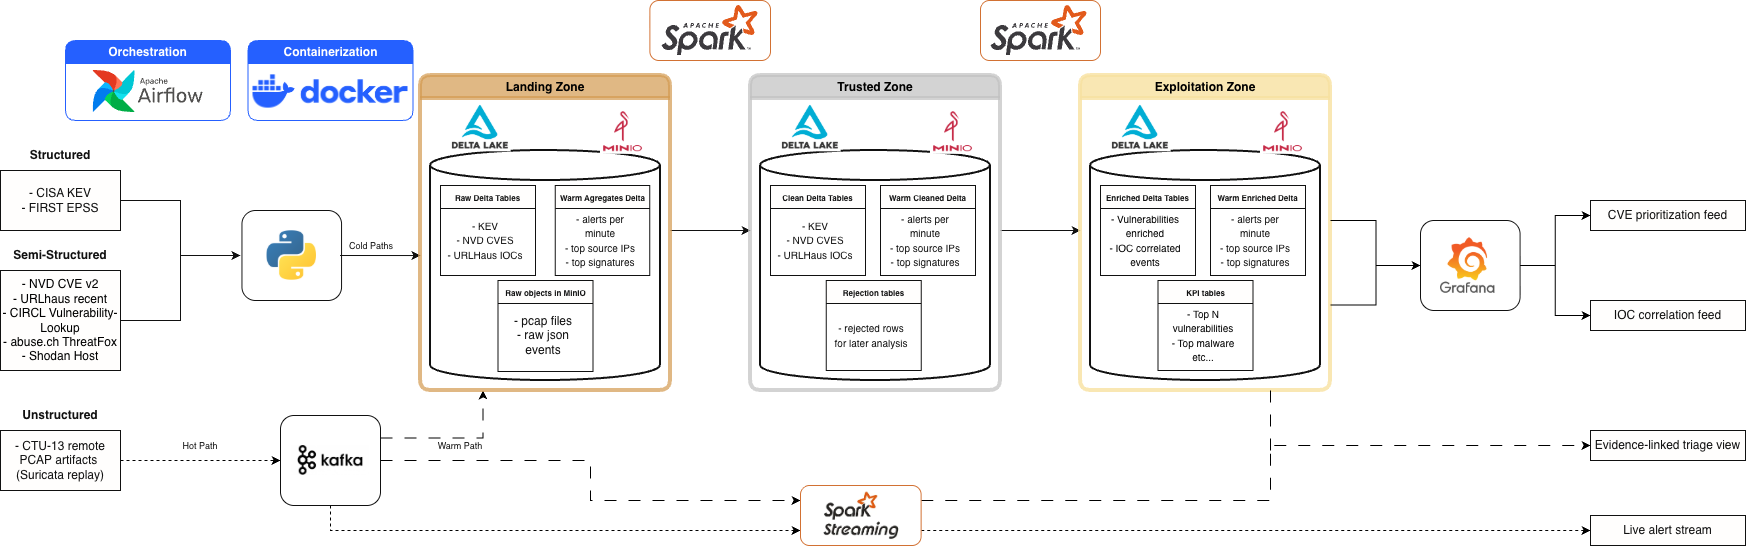
\includegraphics[width=\textwidth,height=0.60\textheight,keepaspectratio]{BDM_P2.drawio.png}%
  }{%
    \fbox{\begin{minipage}[c][0.44\textheight][c]{\textwidth}
      \centering
      \textit{[Architecture diagram -- place \texttt{assets/BDM\_P2.drawio.png} here]}
    \end{minipage}}%
  }
  \caption{CyberSecIntel updated architecture design (P2). Storage remains MinIO + Delta Lake throughout all three pipeline zones. Spark is the sole transformation engine across batch, streaming, and ML paths. The five consumption endpoints cover cold, warm, and hot data paths.}
\end{figure}

\subsection{Technology summary}

\begin{tabularx}{\textwidth}{>{\raggedright\arraybackslash}p{3.0cm}>{\raggedright\arraybackslash}p{2.1cm}X}
\toprule
\textbf{Technology} & \textbf{Zone(s)} & \textbf{Role and justification}\\
\midrule
Apache Spark (PySpark) & Trusted, Exploitation, Consumption & The single transformation engine across all zones. Handles batch ETL (cleaning, joining, correlating, aggregating) for the cold path, Structured Streaming for the warm path, and ML training and inference for the anomaly feed. The Spark SQL Thrift Server exposes Delta tables to Grafana via a persistent SQL endpoint, removing the need for a separate query engine.\\
MinIO + Delta Lake & Landing, Trusted, Exploitation & Same stack as P1, extended to three zones. Delta provides ACID commits, schema enforcement, versioned history, and native Spark integration. All pipeline data, including KPI aggregates, warm enriched alerts, and anomaly flags, remains in MinIO as Delta tables.\\
Apache Kafka & Landing, Consumption & Unchanged from P1. The \code{ids.alerts} topic feeds the warm-path Spark Structured Streaming job; \code{suricata.events} is surfaced directly as the live alert stream.\\
Grafana & Consumption & Dashboarding service that queries exploitation zone Delta tables via the Spark SQL Thrift Server. The only new Docker service introduced in P2.\\
\bottomrule
\end{tabularx}

\subsection{Cold, warm, and hot paths}

The \textbf{cold path} is extended through two new Airflow DAGs running sequentially after the P1 landing DAGs. Each DAG uses Spark to read from the previous zone's Delta tables and write cleaned or enriched tables to the next zone's bucket in MinIO.

The \textbf{warm path} originates at the Kafka \code{ids.alerts} topic published by the P1 Suricata replay pipeline. A Spark Structured Streaming job reads from this topic in micro-batch mode, enriches each alert against the \code{exploitation/vuln\_enriched} Delta table loaded as a static broadcast, and writes results to the warm enriched Delta table in the exploitation zone. The warm aggregates accumulated in the landing zone are also processed by the trusted zone batch ETL, providing a governed historical record alongside the real-time stream.

The \textbf{hot path} (\code{suricata.events}) remains pass-through: raw EVE events are time-critical and already normalized at publish time by the P1 replay pipeline. They are surfaced directly as the live alert stream without further processing.

\subsection{Streaming design}

P1 established a Kafka-backed hot path that publishes Suricata EVE events and IDS alerts to two topics. P2 extends this with a warm-path processing step on \code{ids.alerts}.

\textbf{Hot path (\code{suricata.events}).} Raw EVE events are time-critical and already normalized at publish time. Applying further transformations would add latency without benefit. The hot path therefore remains pass-through, surfaced as the live alert stream.

\textbf{Warm path (\code{ids.alerts}).} IDS alerts have lower volume and tolerate slightly higher latency: enriching an alert with a vulnerability priority score within seconds is sufficient for SOC triage. Spark Structured Streaming reads from the \code{ids.alerts} Kafka topic in micro-batch mode (10-second interval), joins each batch against \code{exploitation/vuln\_enriched} loaded as a static broadcast DataFrame, and writes enriched records to the warm enriched Delta table in \code{s3://exploitation/}.

\textbf{Tool choice.} Spark Structured Streaming is used rather than Kafka Streams or Apache Flink because Spark is already the transformation engine for the batch zones. Reusing it avoids introducing a second framework. The \code{spark-sql-kafka} connector provides native Kafka source support.

\section{Trusted Zone}

\subsection{Design goals and principles}

The trusted zone applies information-preserving transformations: operations that correct representational errors without encoding task-specific assumptions. Concretely, this means deduplication by natural key, type casting, date standardization, structural flattening of nested fields, and validation against expected value ranges or enumerations. It explicitly excludes outlier removal, missing-value imputation, and normalization steps that assume a particular downstream model.

The heuristic applied throughout is: \emph{if two downstream tasks with different requirements consumed this asset, would both benefit from this transformation, or would one of them be harmed?} Only transformations that pass this test are admitted to the trusted zone.

\subsection{Storage}

Each zone holds two primary data threads and one zone-specific object. In the trusted zone: \textbf{Delta clean tables} (\code{s3://trusted/}) contain cleaned versions of each landing zone source, partitioned by source family; \textbf{warm cleaned Delta} contains the cleaned IDS alert aggregates flowing from the landing zone warm aggregates; and \textbf{rejection tables} (\code{s3://trusted/rejected/}) collect rows excluded by mandatory-field or integrity checks, retaining them for audit without dropping them from the pipeline.

\subsection{Cleaning transformations per data type}

\textbf{Structured data (KEV, EPSS).}
\begin{itemize}
  \item \textbf{Deduplication.} KEV on \code{cveID}; EPSS on compound key \code{(cve, date)}.
  \item \textbf{Type casting.} Date strings (\code{dateAdded}, \code{dueDate}) are cast to \code{DateType}. EPSS \code{epss} and \code{percentile} are cast to \code{DoubleType}.
  \item \textbf{Range validation.} EPSS scores outside $[0, 1]$ receive a Boolean \code{\_quality\_warn} flag and are retained rather than dropped, preserving the row for audit.
  \item \textbf{Null enforcement.} Rows with null mandatory fields (\code{cveID}, \code{vulnerabilityName} for KEV; \code{cve}, \code{date} for EPSS) are written to \code{trusted/rejected/} rather than silently discarded.
\end{itemize}

\textbf{Semi-structured data (NVD, URLhaus, CIRCL, ThreatFox).}
\begin{itemize}
  \item \textbf{Schema alignment.} Field names are normalized to snake\_case (\code{cveId} $\to$ \code{cve\_id}, \code{lastModified} $\to$ \code{last\_modified}).
  \item \textbf{Flattening.} NVD CVSS blocks are flattened: \code{metrics.cvssMetricV31[0].cvssData} fields are promoted to top-level columns (\code{cvss\_v3\_score}, \code{cvss\_v3\_vector}, \code{cvss\_v3\_severity}). Missing CVSS blocks produce null columns rather than dropped rows.
  \item \textbf{Missing field defaults.} Optional fields absent in some records receive typed nulls, ensuring a stable column set for downstream Spark jobs.
  \item \textbf{Deduplication.} Natural keys: \code{cve\_id} for NVD and CIRCL; \code{id} for URLhaus and ThreatFox.
  \item \textbf{URL validity.} URLhaus \code{url} values are validated against a basic pattern; invalid entries receive \code{\_quality\_warn=true}.
\end{itemize}

\textbf{Unstructured data (CTU-13 PCAPs, Suricata EVE JSONL).}
\begin{itemize}
  \item \textbf{PCAP integrity.} Each artifact's SHA-256 is recomputed and compared against the sidecar \code{.meta.json} written at landing time. Mismatches set an \code{integrity\_fail} flag in the \code{pcap\_artifacts} Delta table; the file is not deleted.
  \item \textbf{EVE JSONL cleaning.} Suricata EVE records are validated for required fields (\code{event\_type}, \code{timestamp}, \code{src\_ip}). Malformed timestamps receive a sentinel value and a flag. Encoding is standardized to UTF-8. Duplicate events within the same replay run (identified by \code{flow\_id} + \code{timestamp} + \code{event\_type}) are dropped.
\end{itemize}

\textbf{Warm aggregates (IDS alert aggregates).}
The warm aggregates Delta accumulated in the landing zone (alerts per minute, top source IPs, top signatures) are cleaned by the trusted zone batch ETL: deduplication by time window key, type validation on count fields, and null enforcement on the aggregation dimensions. The result is written to the warm cleaned Delta table, providing a governed historical record alongside the real-time warm path.

\subsection{Orchestration}

A new Airflow DAG \code{cybersecintel\_trusted\_zone} depends on completion of both P1 ingestion DAGs. It runs one Spark task per source family and one task for the warm aggregates, writing cleaned Delta tables to \code{s3://trusted/}.

\section{Exploitation Zone}

\subsection{Design goals}

The exploitation zone produces data ready for analyst consumption: pre-joined tables that eliminate repeated join work, IOC-correlated network events, a composite vulnerability priority score, anomaly-flagged flows, and pre-aggregated KPI tables. All data remains in Delta Lake on MinIO, queried by Grafana via the Spark SQL Thrift Server.

\subsection{Storage}

The exploitation zone holds two primary data threads and one zone-specific object. \textbf{Enriched Delta tables} (\code{s3://exploitation/}) contain the joined and correlated analytical assets produced by the cold batch path. \textbf{Warm enriched Delta} contains the continuously updated IDS alerts enriched with CVE context by the Spark Structured Streaming job. \textbf{KPI tables} (\code{s3://exploitation/kpi/}) hold pre-aggregated metrics recomputed by the exploitation DAG on each run and queried directly by Grafana.

\subsection{Data organization and modeling}

\textbf{\code{exploitation/vuln\_enriched} Delta table.}
The central analytical asset is a wide, pre-joined CVE table produced by left-joining \code{trusted/kev}, \code{trusted/nvd}, \code{trusted/epss}, and \code{trusted/circl\_vulnlookup} on \code{cve\_id}. The result is one row per CVE containing KEV exploit status and dates, NVD CVSS scores and description, EPSS probability and percentile, CIRCL CWE and reference counts, and a computed \code{vuln\_priority\_score} column.

\textbf{\code{exploitation/network\_events} Delta table.}
A union of \code{trusted/suricata\_events} and \code{trusted/ids\_alerts} produces a unified network security event log with a consistent schema: event timestamp, type, source and destination IP and port, protocol, alert signature, severity, category, scenario, and origin source. The table is partitioned by ingestion date for efficient time-range scans.

\textbf{\code{exploitation/ioc\_correlations} Delta table.}
A Spark job joins the \code{trusted/threatfox} and \code{trusted/urlhaus} IOC tables against \code{exploitation/network\_events} on source and destination IP addresses and observed URLs where available. Each matching record carries the IOC type (IP, domain, or URL), the associated malware family from ThreatFox, and the original network event context. This table feeds the IOC correlation feed in the consumption layer.

\textbf{\code{exploitation/anomaly\_flags} Delta table.}
A Spark batch job reads \code{exploitation/network\_events} and extracts a feature matrix (alert category, severity, source port, destination port, event count per flow). A trained scikit-learn Isolation Forest model scores each flow; records classified as anomalies by the model are written to this table with their anomaly score and feature values. The trained model artifact is persisted to \code{s3://models/ids\_anomaly\_detector/} for versioning and reuse.

\textbf{KPI tables (\code{s3://exploitation/kpi/}).}
Three pre-aggregated Delta tables are recomputed by the exploitation DAG and queried by Grafana:
\begin{itemize}
  \item \code{kpi\_vuln\_priority\_top50}: the top 50 CVEs by \code{vuln\_priority\_score} with key fields for the CVE prioritization feed.
  \item \code{kpi\_daily\_alert\_counts}: alert count grouped by date, severity, and signature for the alert trend panel.
  \item \code{kpi\_kev\_rolling7d}: count of CVEs added to KEV in the last seven days for the headline stat panel.
\end{itemize}

\subsection{Computed new assets}

\textbf{Vulnerability priority score.}
\[
\textit{priority} = \textit{epss\_score} \times \underbrace{(1.5 \text{ if kev\_listed else } 1.0)}_{\text{exploit confirmation bonus}} \times \frac{\textit{cvss\_v3\_score}}{10}
\]
This composite score encodes three complementary signals: EPSS provides the statistical probability of exploitation in the near term; the KEV bonus elevates CVEs confirmed as actively exploited in the wild; CVSS provides the technical severity weight.

\subsection{Orchestration}

A new Airflow DAG \code{cybersecintel\_exploitation\_zone} depends on \code{cybersecintel\_trusted\_zone}. It runs five tasks: the join task (produces \code{vuln\_enriched}), the union task (produces \code{network\_events}), the IOC correlation task (produces \code{ioc\_correlations}), the ML task (produces \code{anomaly\_flags} and updates \code{s3://models/}), and the KPI task (writes aggregate tables to \code{s3://exploitation/kpi/}). All tasks are idempotent: Delta writes use overwrite mode and KPI tables are fully recomputed on each run.

\section{Data Consumption}

The five consumption endpoints cover all three data paths and deliver distinct business value to SOC analyst workflows. Grafana serves the four cold and warm endpoints by querying exploitation zone Delta tables via the Spark SQL Thrift Server. The live alert stream bypasses Grafana entirely.

\subsection{CVE prioritization feed}

Grafana queries \code{kpi\_vuln\_priority\_top50} and renders a sortable triage table showing the top 50 CVEs by \code{vuln\_priority\_score}, with KEV status, CVSS severity, and EPSS probability. The panel gives SOC analysts a continuously updated ranked list of vulnerabilities to prioritize for patching, combining exploit likelihood, active exploitation evidence, and technical severity into a single score.

\subsection{IOC correlation feed}

Grafana queries \code{exploitation/ioc\_correlations} and displays network events matched against known ThreatFox and URLhaus indicators. Each row shows the matched IOC, its associated malware family, and the source and destination of the network event. Analysts use this feed to identify hosts communicating with known malicious infrastructure without manually cross-referencing threat intelligence sources.

\subsection{ML anomaly feed}

The \code{cybersecintel\_ml\_ids\_anomaly} DAG task runs a two-stage Spark job. In the training stage, Spark reads \code{exploitation/network\_events}, extracts a feature matrix, and trains a scikit-learn Isolation Forest; the model is serialized to \code{s3://models/ids\_anomaly\_detector/}. In the inference stage, Spark loads the model, scores all flows, and writes anomalous records to \code{exploitation/anomaly\_flags}. Grafana queries this table and surfaces flows that deviate from baseline behavior, enabling analysts to detect novel threats that signature-based rules would miss.

\subsection{Alert enrichment feed}

A Spark Structured Streaming job implements the warm-path alert enrichment:
\begin{enumerate}
  \item reads from Kafka \code{ids.alerts} using the \code{spark-sql-kafka} connector in micro-batch mode (10-second interval);
  \item joins each batch against \code{exploitation/vuln\_enriched} loaded as a static broadcast DataFrame, attaching \code{vuln\_priority\_score} and \code{cvss\_v3\_severity};
  \item writes enriched records to the warm enriched Delta table in \code{s3://exploitation/}.
\end{enumerate}
Grafana queries the warm enriched table and displays a live-updating view linking each IDS alert to its CVE context, giving analysts the evidence needed to assess alert severity within seconds of the alert arriving.

\subsection{Live alert stream}

The Kafka topic \code{suricata.events} surfaces raw Suricata EVE events in real time without further processing. Events are already normalized at publish time by the P1 replay pipeline. The live alert stream provides sub-second visibility into network activity and is consumed directly by analyst monitoring tools, bypassing the batch and micro-batch latency of the other endpoints.

\section{Data Governance (Optional)}

\subsection{Data domains and products}

The data in the exploitation zone belongs to four business domains:

\begin{tabularx}{\textwidth}{>{\raggedright\arraybackslash}p{3.2cm}X}
\toprule
\textbf{Domain} & \textbf{Data products}\\
\midrule
Vulnerability Intelligence & \code{exploitation/vuln\_enriched} (Delta), \code{exploitation/kpi/kpi\_vuln\_priority\_top50} (Delta), \code{exploitation/kpi/kpi\_kev\_rolling7d} (Delta)\\
Network Security Events & \code{exploitation/network\_events} (Delta), \code{exploitation/kpi/kpi\_daily\_alert\_counts} (Delta), \code{exploitation/warm\_enriched} (Delta)\\
Threat Intelligence & \code{exploitation/ioc\_correlations} (Delta)\\
ML Artifacts & \code{s3://models/ids\_anomaly\_detector/} (MinIO, versioned by training date), \code{exploitation/anomaly\_flags} (Delta)\\
\bottomrule
\end{tabularx}

\subsection{Detailed data product specification: \texttt{exploitation/vuln\_enriched}}

\begin{tabularx}{\textwidth}{>{\raggedright\arraybackslash}p{3.2cm}X}
\toprule
\textbf{Attribute} & \textbf{Value}\\
\midrule
Name & \code{exploitation/vuln\_enriched}\\
Domain & Vulnerability Intelligence\\
Owner & CyberSecIntel data engineering team\\
Description & Pre-joined CVE enrichment table combining KEV exploit status, NVD CVSS severity, EPSS exploit probability, and CIRCL metadata into one row per CVE for analyst triage.\\
Update cadence & Daily (triggered by \code{cybersecintel\_exploitation\_zone} DAG).\\
Upstream lineage & \code{trusted/kev} $\leftarrow$ join $\to$ \code{trusted/nvd}, \code{trusted/epss}, \code{trusted/circl\_vulnlookup}.\\
Key & \code{cve\_id} (unique per row).\\
Quality checks & Non-null \code{cve\_id}; \code{epss\_score} $\in [0,1]$; \code{cvss\_v3\_score} $\in [0,10]$ or null; \code{vuln\_priority\_score} $\geq 0$.\\
Access policy & Readable by analysts, streaming job, and ML DAG task; write access restricted to the exploitation DAG service account.\\
Retention & Overwritten on each run; Delta Lake transaction log retained for 30 days to allow rollback.\\
\bottomrule
\end{tabularx}

\subsection{Lineage tracking}

Each Spark job in the trusted and exploitation DAGs appends one row to a lineage Delta table at \code{s3://exploitation/lineage/} with columns: \code{run\_id}, \code{dag\_id}, \code{task\_id}, \code{source\_paths}, \code{target\_path}, \code{transformation\_name}, \code{rows\_read}, \code{rows\_written}, \code{rows\_rejected}, \code{started\_at}, \code{finished\_at}. Storing lineage in Delta keeps all pipeline metadata within the same storage layer, and the table is directly queryable by Grafana or Spark for pipeline health monitoring.

\section{Constraint Coverage}

{\small
\begin{tabularx}{\textwidth}{>{\raggedright\arraybackslash}p{3.3cm}X}
\toprule
\textbf{P2 constraint} & \textbf{Design response}\\
\midrule
C1 -- Trusted Zone design & Storage (\code{s3://trusted/} + Delta), technology (Spark), and per-source cleaning transformations defined in Section~2. Three storage objects per zone: Delta clean tables, warm cleaned Delta, rejection tables.\\
C2 -- Trusted Zone implementation & Spark jobs per source family and warm aggregates; Airflow DAG \code{cybersecintel\_trusted\_zone}; rejection side table at \code{trusted/rejected/}; lineage records in Delta.\\
C3 -- Exploitation Zone design & Five Delta assets defined in Section~3: \code{vuln\_enriched}, \code{network\_events}, \code{ioc\_correlations}, \code{anomaly\_flags}, and KPI tables, each with join keys, schema, and computed columns.\\
C4 -- Exploitation Zone implementation & Spark ETL with five idempotent tasks; Delta overwrite mode; KPI tables fully recomputed per run; DAG \code{cybersecintel\_exploitation\_zone}.\\
C5 -- Consumption design and implementation & Five endpoints: CVE prioritization feed, IOC correlation feed, ML anomaly feed, and alert enrichment feed (all via Grafana querying Delta through Spark SQL), plus live alert stream (Kafka hot path, pass-through). Described in Section~4.\\
C6 -- Architecture design & Updated diagram (Figure~1) shows all zones, storage objects, data paths (cold/warm/hot), and consumption endpoints. Section~1 explains the Option~1 rationale and per-tool justification.\\
C7 -- Orchestration and containerization & Two new Airflow DAGs extend P1 orchestration. Grafana is the only new Docker service; MinIO, Spark, and Kafka are reused.\\
C8 -- Organization & Code organized under \code{trusted/}, \code{exploitation/}, and \code{consumption/} top-level directories, each with per-source or per-task scripts.\\
\bottomrule
\end{tabularx}
}

\section{References}

{\small
\begin{itemize}
  \item Apache Spark documentation: \url{https://spark.apache.org/docs/latest/}
  \item Spark SQL Thrift Server: \url{https://spark.apache.org/docs/latest/sql-distributed-sql-engine.html}
  \item Delta Lake project: \url{https://delta.io/}
  \item MinIO object storage: \url{https://min.io/}
  \item Grafana documentation: \url{https://grafana.com/docs/}
  \item Apache Kafka documentation: \url{https://kafka.apache.org/documentation/}
  \item Apache Airflow documentation: \url{https://airflow.apache.org/docs/}
  \item scikit-learn Isolation Forest: \url{https://scikit-learn.org/stable/modules/generated/sklearn.ensemble.IsolationForest.html}
  \item P1 source references (KEV, NVD, EPSS, URLhaus, CIRCL, ThreatFox, CTU-13): see P1 Final Delivery, Section~2.3.
\end{itemize}
}

\end{document}
